\setmodule{7}

%BEGIN_FOLD % ====>>_____ Занятие 1 _____<<====
\begin{class}[number=1]
	\begin{listofex}
		\item Два ребра прямоугольного параллелепипеда, выходящие из одной вершины, равны \(1, 2\). Объем параллелепипеда равен \(6\). Найдите площадь его поверхности.
		\item Два ребра прямоугольного параллелепипеда равны \(7\) и \(4\), а объём параллелепипеда равен \(140\). Найдите площадь поверхности этого параллелепипеда.
		\item 
		\begin{minipage}[t]{\bodywidth}
			В прямоугольном параллелепипеде \(ABCDA_1B_1C_1D_1\) рёбра \(AB, BC\) и диагональ боковой грани \(BC_1\) равны соответственно \(7, \) \( 3\) и \(3\sqrt{5}\). Найдите объём параллелепипеда \(ABCDA_1B_1C_1D_1\).
		\end{minipage}
		\hspace{0.02\linewidth}
		\begin{minipage}[t]{\picwidth}
			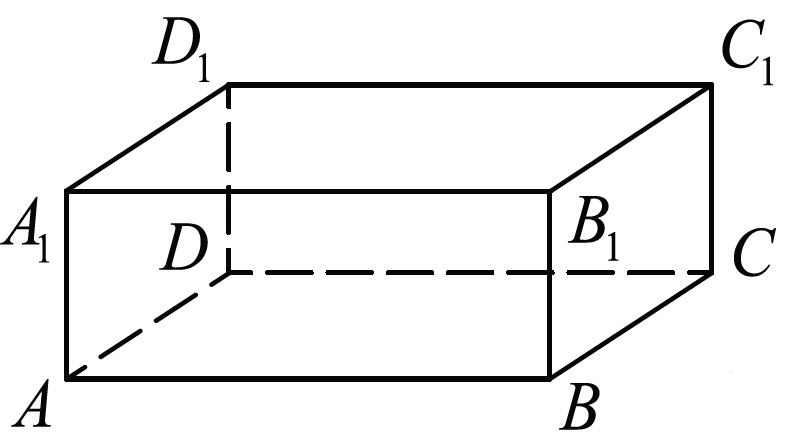
\includegraphics[align=t, width=\linewidth]{\picpath/G101M9L1-1}
		\end{minipage}
		\item 
		\begin{minipage}[t]{\bodywidth}
			В прямоугольном параллелепипеде \(ABCDA_1B_1C_1D_1\) рёбра \(CD, CB\) и диагональ \(CD_1\) боковой грани равны соответственно \(2, 4\) и \(2\sqrt{10}\). Найдите площадь поверхности параллелепипеда \(ABCDA_1B_1C_1D_1\).
		\end{minipage}
		\hspace{0.02\linewidth}
		\begin{minipage}[t]{\picwidth}
			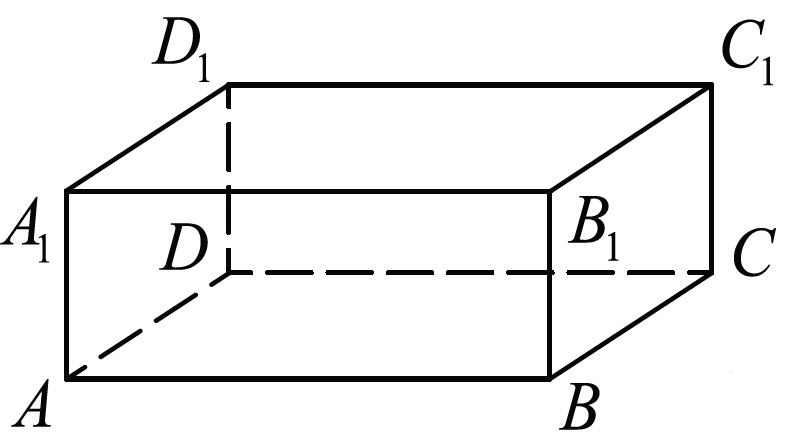
\includegraphics[align=t, width=\linewidth]{\picpath/G101M9L1-1}
		\end{minipage}
		\item Основанием прямой треугольной призмы служит прямоугольный треугольник с катетами \(6\) и \(8\), боковое ребро равно \(5\). Найдите объем призмы.
		\item В основании прямой призмы лежит прямоугольный треугольник, один из катетов которого равен \(2\), а гипотенуза равна \(\sqrt{53}\). Найдите объём призмы, если её высота равна \(3\).
		\item В основании прямой призмы лежит прямоугольный треугольник, катеты которого равны \(11\) и \(5\). Найдите объём призмы, если её высота равна \(4\).
		\item 
		\begin{minipage}[t]{\bodywidth}
			Стороны основания правильной шестиугольной пирамиды равны \(10\), боковые ребра равны \(13\). Найдите площадь боковой поверхности этой пирамиды.
		\end{minipage}
		\hspace{0.02\linewidth}
		\begin{minipage}[t]{\picwidth}
			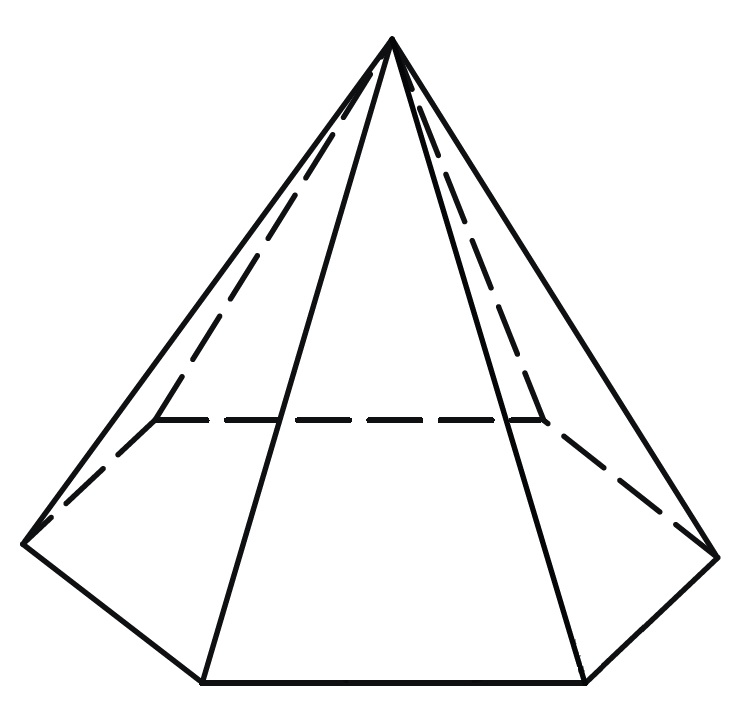
\includegraphics[align=t, width=\linewidth]{\picpath/G101M9L1-2}
		\end{minipage}
		\item 
		\begin{minipage}[t]{\bodywidth}
			Основанием пирамиды является прямоугольник со сторонами \(3\) и \(4\). Ее объем равен \(16\). Найдите высоту этой пирамиды.
		\end{minipage}
		\hspace{0.02\linewidth}
		\begin{minipage}[t]{\picwidth}
			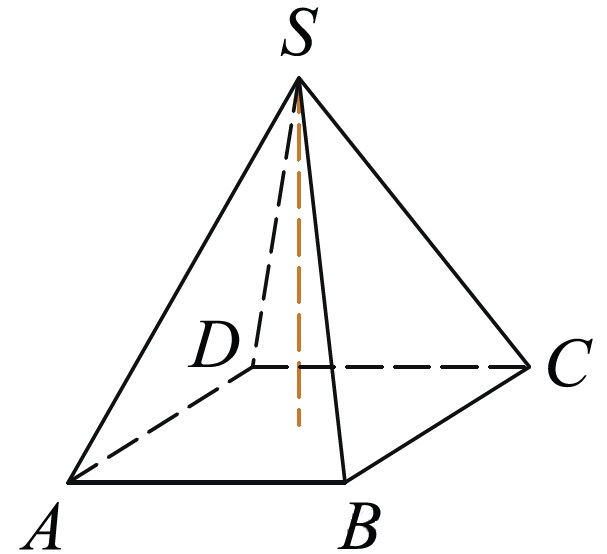
\includegraphics[align=t, width=\linewidth]{\picpath/G101M9L1-3}
		\end{minipage}
		\item 
		\begin{minipage}[t]{\bodywidth}
			Основанием пирамиды является прямоугольник со сторонами \(4\) и \(5\). Ее объем равен \(80\). Найдите высоту этой пирамиды.
		\end{minipage}
		\hspace{0.02\linewidth}
		\begin{minipage}[t]{\picwidth}
			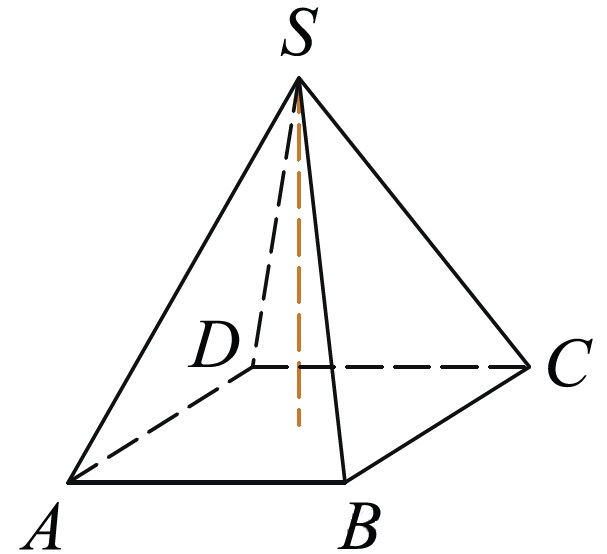
\includegraphics[align=t, width=\linewidth]{\picpath/G101M9L1-3}
		\end{minipage}
		\item 
		\begin{minipage}[t]{\bodywidth}
			Найдите объём правильной четырёхугольной пирамиды, сторона основания которой равна \(4\), а боковое ребро равно \(\sqrt{17}\).
		\end{minipage}
		\hspace{0.02\linewidth}
		\begin{minipage}[t]{\picwidth}
			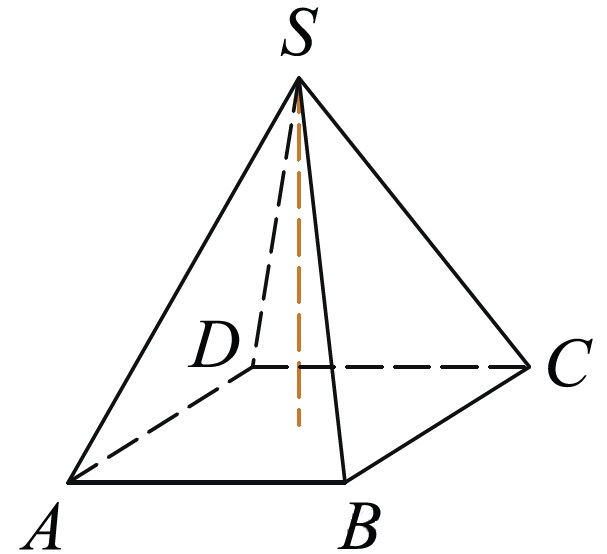
\includegraphics[align=t, width=\linewidth]{\picpath/G101M9L1-3}
		\end{minipage}
		\item 
		\begin{minipage}[t]{\bodywidth}
			В основании пирамиды \(SABC\) лежит правильный треугольник \(ABC\) со стороной \(10\), а боковое ребро \(SA\) перпендикулярно основанию и равно Найдите объём пирамиды \(SABC\).
		\end{minipage}
		\hspace{0.02\linewidth}
		\begin{minipage}[t]{\picwidth}
			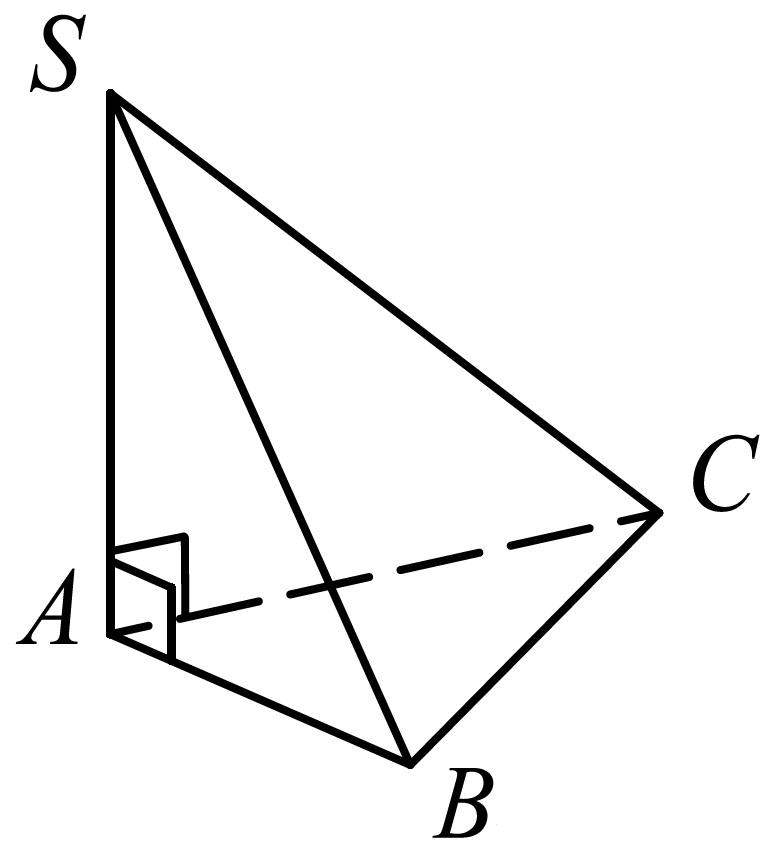
\includegraphics[align=t, width=\linewidth]{\picpath/G101M9L1-4}
		\end{minipage}
		\item 
		\begin{minipage}[t]{\bodywidth}
			В треугольной пирамиде \(ABCD\) рёбра \(AB, AC\) и \(AD\) взаимно перпендикулярны. Найдите объём этой пирамиды, если \(AB = 6, AC = 18\) и \(AD = 8\).
		\end{minipage}
		\hspace{0.02\linewidth}
		\begin{minipage}[t]{\picwidth}
			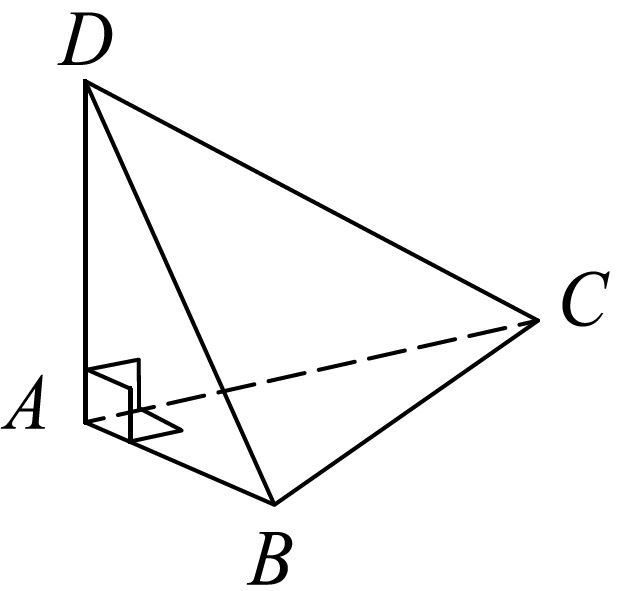
\includegraphics[align=t, width=\linewidth]{\picpath/G101M9L1-5}
		\end{minipage}
		\newpage
		\item Стороны основания правильной треугольной пирамиды равны \(16\), а боковые рёбра равны \(10\). Найдите площадь боковой поверхности пирамиды.
		\item Даны два цилиндра. Радиус основания и высота первого равны соответственно \(4\) и \(18\), а второго --- \(2\) и \(3\). Во сколько раз площадь боковой поверхности первого цилиндра больше площади боковой поверхности второго?
		
		
		%\item 
		%\begin{minipage}[t]{\bodywidth}
		%	
		%\end{minipage}
		%\hspace{0.02\linewidth}
		%\begin{minipage}[t]{\picwidth}
		%	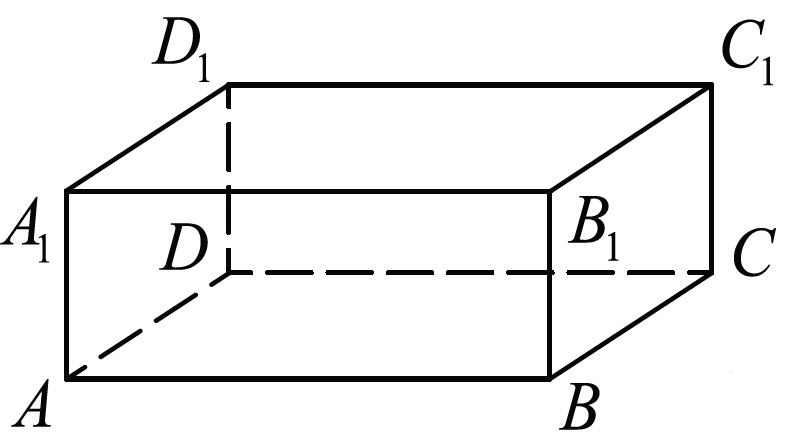
\includegraphics[align=t, width=\linewidth]{\picpath/G101M9L1-1}
		%\end{minipage}
	\end{listofex}
\end{class}
%END_FOLD

%BEGIN_FOLD % ====>>_____ Занятие 2 _____<<====
\begin{class}[number=2]
	\begin{listofex}
		\item Занятие 2
	\end{listofex}
\end{class}
%END_FOLD

%BEGIN_FOLD % ====>>_ Домашняя работа 1 _<<====
\begin{homework}[number=1]
	\begin{listofex}
		
		\item Основанием прямой треугольной призмы служит прямоугольный треугольник с катетами \(12\) и \(5\), боковое ребро равно \(6\). Найдите объем призмы.
		\item В основании прямой призмы лежит прямоугольный треугольник, катеты которого равны по \(12\). Найдите объём призмы, если её высота равна \(2\).
		\item Два ребра прямоугольного параллелепипеда, выходящие из одной вершины, равны \(4, 6\). Объем параллелепипеда равен \(48\). Найдите площадь его поверхности.
		\item 
		\begin{minipage}[t]{\bodywidth}
			В основании пирамиды \(SABC\) лежит правильный треугольник \(ABC\) со стороной \(4\), а боковое ребро \(SA\) перпендикулярно основанию и равно \(7\) Найдите объём пирамиды \(SABC\).
		\end{minipage}
		\hspace{0.02\linewidth}
		\begin{minipage}[t]{\picwidth}
			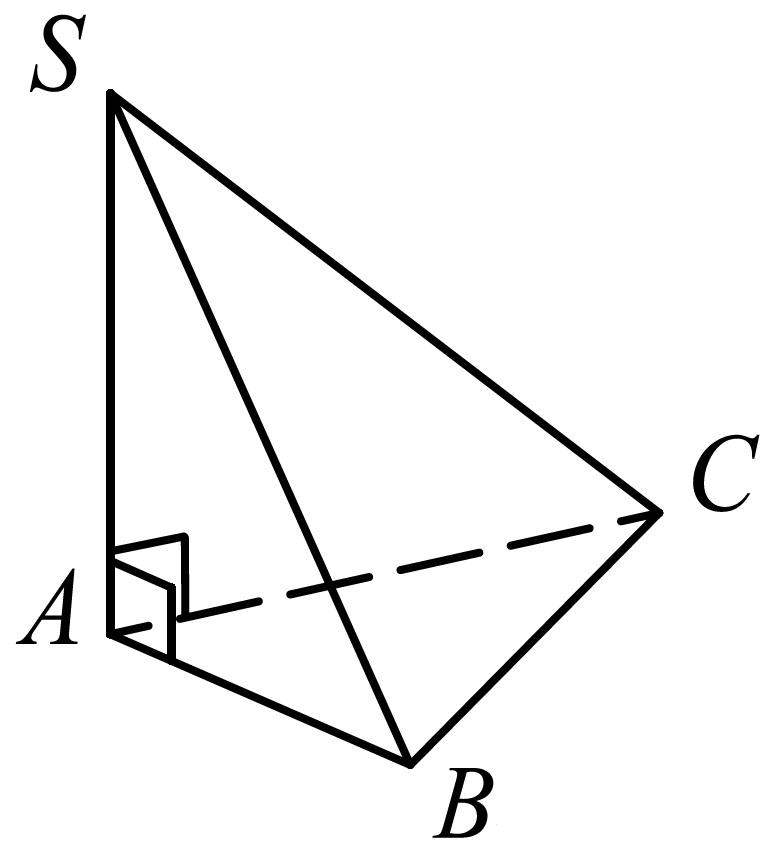
\includegraphics[align=t, width=\linewidth]{\picpath/G101M9L1-4}
		\end{minipage}
		\item Объём конуса равен \(50\pi \), а его высота равна \(6\). Найдите радиус основания конуса.
		\item Даны два конуса. Радиус основания и образующая первого конуса равны, соответственно, \(2\) и \(4\), а второго --- \(6\) и \(8\). Во сколько раз площадь боковой поверхности второго конуса больше площади боковой поверхности первого?
		\item Даны два конуса. Радиус основания и высота первого конуса равны соответственно \(9\) и \(2\), а второго --- \(3\) и \(3\). Во сколько раз объём первого конуса больше объёма второго?
		\item Даны два шара с радиусами \(5\) и \(1\). Во сколько раз площадь поверхности первого шара больше площади поверхности второго?
		\item Даны два шара с радиусами \(4\) и \(1\). Во сколько раз объём большего шара больше объёма другого?
		\item Даны два шара с радиусами \(9\) и \(3\). Во сколько раз площадь поверхности большего шара больше площади поверхности меньшего?
	\end{listofex}
\end{homework}
%END_FOLD

%BEGIN_FOLD % ====>>_____ Занятие 3 _____<<====
\begin{class}[number=3]
	\begin{listofex}
		\item Стороны основания правильной треугольной пирамиды равны \(16\), а боковые рёбра равны \(10\). Найдите площадь боковой поверхности пирамиды.
		\item Даны два цилиндра. Радиус основания и высота первого равны соответственно \(4\) и \(18\), а второго --- \(2\) и \(3\). Во сколько раз площадь боковой поверхности первого цилиндра больше площади боковой поверхности второго?
		\item Объём конуса равен \(108\pi \), а его высота равна \(3\). Найдите радиус основания конуса.
		\item Даны два конуса. Радиус основания и образующая первого конуса равны, соответственно, \(5\) и \(4\), а второго --- \(10\) и \(8\). Во сколько раз площадь боковой поверхности второго конуса больше площади боковой поверхности первого?
		\item Даны два конуса. Радиус основания и высота первого конуса равны соответственно \(5\) и \(10\), а второго --- \(3\) и \(2\). Во сколько раз объём первого конуса больше объёма второго?
		\item Даны два шара с радиусами \(8\) и \(11\). Во сколько раз площадь поверхности первого шара больше площади поверхности второго?
		\item Даны два шара с радиусами \(2\) и \(8\). Во сколько раз объём большего шара больше объёма другого?
		\item Даны два шара с радиусами \(6\) и \(14\). Во сколько раз площадь поверхности большего шара больше площади поверхности меньшего?
		\item Теплоход проходит по течению реки до пункта назначения \(255\) км и после стоянки возвращается в пункт отправления. Найдите скорость теплохода в неподвижной воде, если скорость течения равна \(1\) км/ч, стоянка длится \(2\) часа, а в пункт отправления теплоход возвращается через \(34\) часа после отплытия из него. Ответ дайте в км/ч.
		\item Моторная лодка в \(10:00\) вышла из пункта \(A\) в пункт \(B\), расположенный в \(30\) км от \(A\). Пробыв в пункте \(B\) \(2\) часа \(30\) минут, лодка отправилась назад и вернулась в пункт \(A\) в \(18:00\). Определите (в км/ч) собственную скорость лодки, если известно, что скорость течения реки \(1\) км/ч.
		\item Теплоход, скорость которого в неподвижной воде равна \(25\) км/ч, проходит по течению реки и после стоянки возвращается в исходный пункт. Скорость течения равна \(3\) км/ч, стоянка длится \(5\) часов, а в исходный пункт теплоход возвращается через \(30\) часов после отплытия из него. Сколько километров прошел теплоход за весь рейс?
		\item Теплоход проходит по течению реки до пункта назначения \(200\) км и после стоянки возвращается в пункт отправления. Найдите скорость течения, если скорость теплохода в неподвижной воде равна \(15\) км/ч, стоянка длится \(10\) часов, а в пункт отправления теплоход возвращается через \(40\) часов после отплытия из него. Ответ дайте в км/ч.
		\item Пристани \(A\) и \(B\) расположены на озере, расстояние между ними \(390\) км. Баржа отправилась с постоянной скоростью из \(A\) в \(B\). На следующий день после прибытия она отправилась обратно со скоростью на \(3\) км/ч больше прежней, сделав по пути остановку на \(9\) часов. В результате она затратила на обратный путь столько же времени, сколько на путь из \(A\) в \(B\). Найдите скорость баржи на пути из \(A\) в \(B\). Ответ дайте в км/ч.
		\item Моторная лодка прошла против течения реки \(112\) км и вернулась в пункт отправления, затратив на обратный путь на \(6\) часов меньше. Найдите скорость течения, если скорость лодки в неподвижной воде равна \(11\) км/ч. Ответ дайте в км/ч.
	\end{listofex}
\end{class}
%END_FOLD

%BEGIN_FOLD % ====>>_____ Занятие 4 _____<<====
\begin{class}[number=4]
	\begin{listofex}
		\item Найдите корень уравнения: \( 2^{2x-3}=2^{2x-2} \).
		\item Найдите корень уравнения: \( 2^{4-2x}=64 \).
		\item Найдите корень уравнения: \( 5^{x-7}=\dfrac{ 1 }{ 125 } \).
		\item Найдите корень уравнения: \( \left( \dfrac{ 1 }{ 3 } \right)^{x-8}=\dfrac{ 1 }{ 9 } \).
		\item Найдите корень уравнения: \( \left( \dfrac{ 1 }{ 2 } \right)^{6-2x}=4 \).
		\item Найдите корень уравнения: \( 16^{x-9}=0,5 \).
		\item Найдите корень уравнения: \( \left( \dfrac{ 1 }{ 9 } \right)^{x-13}=3 \).
		\item Найдите корень уравнения: \( 9^{-5+x}=729 \).
		
		
		
		
		\item Пристани \(A\) и \(B\) расположены на озере, расстояние между ними \(390\) км. Баржа отправилась с постоянной скоростью из \(A\) в \(B\). На следующий день после прибытия она отправилась обратно со скоростью на \(3\) км/ч больше прежней, сделав по пути остановку на \(9\) часов. В результате она затратила на обратный путь столько же времени, сколько на путь из \(A\) в \(B\). Найдите скорость баржи на пути из \(A\) в \(B\). Ответ дайте в км/ч.
		\item Моторная лодка прошла против течения реки \(112\) км и вернулась в пункт отправления, затратив на обратный путь на \(6\) часов меньше. Найдите скорость течения, если скорость лодки в неподвижной воде равна \(11\) км/ч. Ответ дайте в км/ч.
		
		\item На изготовление \(475\) деталей первый рабочий тратит на \(6\) часов меньше, чем второй рабочий на изготовление \(550\) таких же деталей. Известно, что первый рабочий за час делает на \(3\) детали больше, чем второй. Сколько деталей в час делает первый рабочий?
		\item Первая труба пропускает на \(3\) литра воды в минуту меньше, чем вторая. Сколько литров воды в минуту пропускает первая труба, если резервуар объемом \(108\) литров она заполняет на \(3\) минуты дольше, чем вторая труба?
		\item Первый насос наполняет бак за \(20\) минут, второй --- за \(30\) минут, а третий --- за \(1\) час. За сколько минут наполнят бак три насоса, работая одновременно?
		\item Игорь и Паша красят забор за \(9\) часов. Паша и Володя красят этот же забор за \(12\) часов, а Володя и Игорь --- за \(18\) часов. За сколько часов мальчики покрасят забор, работая втроем?
		\item Заказ на \(156\) деталей первый рабочий выполняет на \(1\) час быстрее, чем второй. Сколько деталей за час изготавливает первый рабочий, если известно, что он за час изготавливает на \(1\) деталь больше второго?
		\item Первый и второй насосы наполняют бассейн за \(9\) минут, второй и третий --- за \(14\) минут, а первый и третий --- за \(18\) минут. За сколько минут эти три насоса заполнят бассейн, работая вместе?
		
		
		
		
	\end{listofex}
\end{class}
%END_FOLD

%BEGIN_FOLD % ====>>_ Домашняя работа 2 _<<====
\begin{homework}[number=2]
	\begin{listofex}
		\item Найдите корень уравнения:
		\begin{tasks}(2)
			\task \( 6^{2x-6}=216 \)
			\task \( \left( \dfrac{ 1 }{ 8 } \right)^{x-3}=512 \)
			\task \( \left( \dfrac{ 1 }{ 2 } \right)^{0,5x+2}=64 \)
			\task \( 5^{14x-3}=625 \)
		\end{tasks}
		\item Два велосипедиста одновременно отправились в \(240\)-километровый пробег. Первый ехал со скоростью, на \(1\) км/ч большей, чем скорость второго, и прибыл к финишу на \(1\) час раньше второго. Найти скорость велосипедиста, пришедшего к финишу первым. Ответ дайте в км/ч
		\item Баржа в \(10:00\) вышла из пункта \(A\) в пункт \(B\), расположенный в \(15\) км от \(A\). Пробыв в пункте B \(1\) час \(20\) минут, баржа отправилась назад и вернулась в пункт \(A\) в \(16:00\) того же дня. Определите (в км/час) скорость течения реки, если известно, что собственная скорость баржи равна \(7\) км/ч.
		\item Заказ на \(156\) деталей первый рабочий выполняет на \(1\) час быстрее, чем второй. Сколько деталей в час делает первый рабочий, если известно, что он за час делает на \(1\) деталь больше?
		%\item На изготовление \(99\) деталей первый рабочий тратит на \(2\) часа меньше, чем второй рабочий на изготовление \(110\) таких же деталей. Известно, что первый рабочий за час делает на \(1\) деталь больше, чем второй. Сколько деталей в час делает второй рабочий?
		\item На изготовление \(99\) деталей первый рабочий тратит на \(2\) часа меньше, чем второй рабочий на изготовление \(110\) таких же деталей. Известно, что первый рабочий за час делает на \(1\) деталь больше, чем второй. Сколько деталей в час делает второй рабочий?
		\item Первая труба пропускает на \(8\) литров воды в минуту меньше, чем вторая. Сколько литров воды в минуту пропускает первая труба, если резервуар объемом \(660\) литров она заполняет на \(11\) минут дольше, чем вторая труба заполняет резервуар объемом \(570\) литров?
	\end{listofex}
\end{homework}
%END_FOLD

%BEGIN_FOLD % ====>>_____ Занятие 5 _____<<====
\begin{class}[number=5]
	\begin{listofex}
		%1 3 5 10 11 15 16 17 18 19 20 22
		\item Заказ на \(110\) деталей первый рабочий выполняет на \(1\) час быстрее, чем второй. Сколько деталей в час делает второй рабочий, если известно, что первый за час делает на \(1\) деталь больше?
		\item На изготовление \(475\) деталей первый рабочий тратит на 6 часов меньше, чем второй рабочий на изготовление 550 таких же деталей. Известно, что первый рабочий за час делает на 3 детали больше, чем второй. Сколько деталей в час делает первый рабочий?
		\item Двое рабочих, работая вместе, могут выполнить работу за \(12\) дней. За сколько дней, работая отдельно, выполнит эту работу первый рабочий, если он за два дня выполняет такую же часть работы, какую второй --- за три дня?
		\item Первая труба пропускает на \(1\) литр воды в минуту меньше, чем вторая. Сколько литров воды в минуту пропускает первая труба, если резервуар объемом \(110\) литров она заполняет на \(1\) минуту дольше, чем вторая труба?
		\item Каждый из двух рабочих одинаковой квалификации может выполнить заказ за \(15\) часов. Через \(3\) часа после того, как один из них приступил к выполнению заказа, к нему присоединился второй рабочий, и работу над заказом они довели до конца уже вместе. Сколько часов потребовалось на выполнение всего заказа?
		\item Один мастер может выполнить заказ за \(12\) часов, а другой --- за \(6\) часов. За сколько часов выполнят заказ оба мастера, работая вместе?
		\item Игорь и Паша красят забор за \(9\) часов. Паша и Володя красят этот же забор за \(12\) часов, а Володя и Игорь --- за \(18\) часов. За сколько часов мальчики покрасят забор, работая втроем?
		\item Две трубы наполняют бассейн за \(3\) часа \(36\) минут, а одна первая труба наполняет бассейн за \(6\) часов. За сколько часов наполняет бассейн одна вторая труба?
		\item Первая труба наполняет резервуар на \(6\) минут дольше, чем вторая. Обе трубы наполняют этот же резервуар за \(4\) минуты. За сколько минут наполняет этот резервуар одна вторая труба?
		\item В помощь садовому насосу, перекачивающему \(5\) литров воды за \(2\) минуты, подключили второй насос, перекачивающий тот же объем воды за \(3\) минуты. Сколько минут эти два насоса должны работать совместно, чтобы перекачать \(25\) литров воды?
		\item Петя и Ваня выполняют одинаковый тест. Петя отвечает за час на \(8\) вопросов теста, а Ваня --- на \(9\). Они одновременно начали отвечать на вопросы теста, и Петя закончил свой тест позже Вани на \(20\) минут. Сколько вопросов содержит тест?
		\item Плиточник должен уложить \(175\) м\(^2\) плитки. Если он будет укладывать на \(10\) м\(^2\) в день больше, чем должен, то закончит работу на \(2\) дня раньше. Сколько квадратных метров плитки в день должен укладывать плиточник?
		\item Первый и второй насосы наполняют бассейн за \(9\) минут, второй и третий --- за \(14\) минут, а первый и третий --- за \(18\) минут. За сколько минут эти три насоса заполнят бассейн, работая вместе?
		\item Первый и второй насосы наполняют бассейн за \(10\) минут, второй и третий --- за \(15\) минут, а первый и третий --- за \(24\) минуты. За сколько минут три эти насоса заполнят бассейн, работая вместе?
	\end{listofex}
\end{class}
%END_FOLD

%BEGIN_FOLD % ====>>_____ Занятие 6 _____<<====
\begin{class}[number=6]
	\begin{listofex}
		\item Каждому из четырёх неравенств в левом столбце соответствует одно из решений в правом столбце. Установите соответствие между неравенствами и их решениями. \\
		\begin{minipage}[t]{0.45\linewidth}
			\begin{tasks}
				\task \( x^2+8x+15 \ge 0 \)
				\task \( x^2 - 8x + 15 \ge 0 \)
				\task \( x^2 - 14x - 15 \le 0 \)
				\task \( x^2 + 14x - 15 \le 0 \)
			\end{tasks}
		\end{minipage}
		\hspace{0.02\linewidth}
		\begin{minipage}[t]{0.45\linewidth}
			\begin{tasks}
				\task \( (- \infty; 3 ] \cup [5; + \infty ) \)
				\task \([-1; 15]  \)
				\task \(  (- \infty; -5 ] \cup [-3; + \infty ) \)
				\task \( [-15; 1] \)
			\end{tasks}
		\end{minipage}
		
		\item Каждому из четырёх неравенств в левом столбце соответствует одно из решений в правом столбце. Установите соответствие между неравенствами и их решениями. \\
	\begin{minipage}[t]{0.45\linewidth}
		\begin{tasks}
			\task \( (x-1)^2(x-5) < 0 \)
			\task \( (x-1)(x-5) < 0 \)
			\task \( \dfrac{ x-1 }{ x-5 }>0 \)
			\task \( \dfrac{ (x-5)^2 }{ x-1 }>0 \)
		\end{tasks}
	\end{minipage}
	\hspace{0.02\linewidth}
	\begin{minipage}[t]{0.45\linewidth}
		\begin{tasks}
			\task \( (- \infty;1) \cup (1; 5) \)
			\task \( (1;5) \)
			\task \( (1;5) \cup (5; + \infty) \)
			\task \( (-\infty;1) \cup (5; +\infty) \)
		\end{tasks}
	\end{minipage}
		
		\item Каждому из четырёх неравенств в левом столбце соответствует одно из решений в правом столбце. Установите соответствие между неравенствами и их решениями. \\
		\begin{minipage}[t]{0.45\linewidth}
			\begin{tasks}
				\task \( \dfrac{ 1 }{ (x-2)(x-3) } > 0 \)
				\task \( 3^{-x+3} > 3 \)
				\task \( \log_3 x > 1 \)
				\task \( \dfrac{ x-3 }{ x-2 } < 0 \)
			\end{tasks}
		\end{minipage}
		\hspace{0.02\linewidth}
		\begin{minipage}[t]{0.45\linewidth}
			\begin{tasks}
				\task \( x<2 \) или \(x>3\)
				\task \( 2<x<3 \)
				\task \( x<2 \)
				\task \( x>3 \)
			\end{tasks}
		\end{minipage}
		
		\item Каждому из четырёх неравенств в левом столбце соответствует одно из решений в правом столбце. Установите соответствие между неравенствами и их решениями. \\
		\begin{minipage}[t]{0.45\linewidth}
			\begin{tasks}
				\task \( (x-3)(x-6) < 0 \)
				\task \( \dfrac{ (x-6)^2 }{ x-3 } >0 \)
				\task \( \dfrac{ x-3 }{ x-6 } > 0 \)
				\task \( (x-3)^2(x-6) < 0 \)
			\end{tasks}
		\end{minipage}
		\hspace{0.02\linewidth}
		\begin{minipage}[t]{0.45\linewidth}
			\begin{tasks}
				\task \( (3;6) \)
				\task \( (-\infty; 3) \cup (6; + \infty) \)
				\task \( (3;6) \cup (6; +\infty) \)
				\task \( (- \infty; 3) \cup (3;6) \)
			\end{tasks}
		\end{minipage}
		
		\item Каждому из четырёх неравенств в левом столбце соответствует одно из решений в правом столбце. Установите соответствие между неравенствами и их решениями. \\
		\begin{minipage}[t]{\bodywidth}
			\begin{tasks}
				\task \( 2^x \ge 4 \)
				\task \( 0,5^x \ge 4 \)
				\task \( 0,5^x \le 4 \)
				\task \( 2^x \le 4 \)
			\end{tasks}
		\end{minipage}
		\hspace{0.02\linewidth}
		\begin{minipage}[t]{\picwidth}
			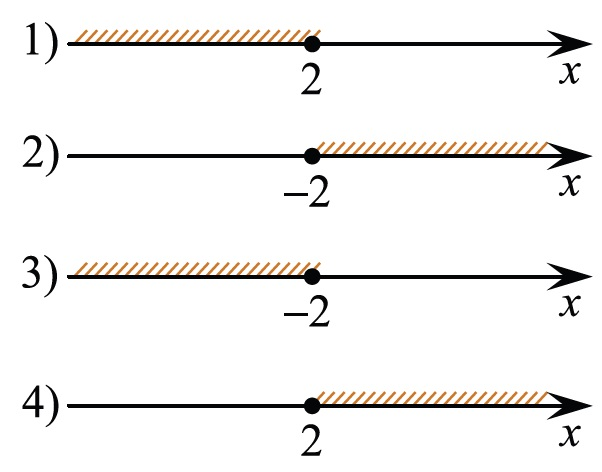
\includegraphics[align=t, width=\linewidth]{\picpath/G101M9L6-1}
		\end{minipage}
		
		\item Каждому из четырёх неравенств в левом столбце соответствует одно из решений в правом столбце. Установите соответствие между неравенствами и их решениями. \\
		\begin{minipage}[t]{\bodywidth}
			\begin{tasks}
				\task \( 0,5^x \ge 4 \)
				\task \( 2^x \ge 4 \)
				\task \( 0,5^x \le 4 \)
				\task \( 2^x \le 4 \)
			\end{tasks}
		\end{minipage}
		\hspace{0.02\linewidth}
		\begin{minipage}[t]{\picwidth}
			\begin{tasks}
				\task \( [-2; +\infty) \)
				\task \( [2; +\infty) \)
				\task \( (- \infty; 2] \)
				\task \( (- \infty; -2] \)
			\end{tasks}
		\end{minipage}
		
		\item Каждому из четырёх неравенств в левом столбце соответствует одно из решений в правом столбце. Установите соответствие между неравенствами и их решениями. \\
		\begin{minipage}[t]{\bodywidth}
			\begin{tasks}
				\task \( 2^x \ge 2 \)
				\task \( 0,5^x \ge 2 \)
				\task \( 0,5^x \le 2\)
				\task \( 2^x \le 2 \)
			\end{tasks}
		\end{minipage}
		\hspace{0.02\linewidth}
		\begin{minipage}[t]{\picwidth}
			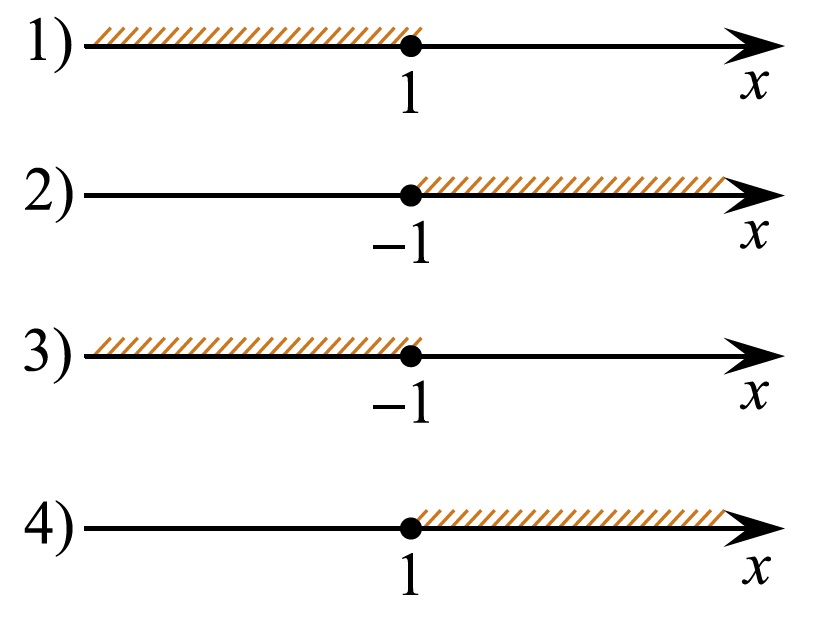
\includegraphics[align=t, width=\linewidth]{\picpath/G101M9L6-2}
		\end{minipage}
		
		\item Каждому из четырёх неравенств в левом столбце соответствует одно из решений в правом столбце. Установите соответствие между неравенствами и их решениями. \\
		\begin{minipage}[t]{\bodywidth}
			\begin{tasks}
				\task \( \log_3 < -1 \)
				\task \( \log_3 x > 1 \)
				\task \( \log_3 x < 1  \)
				\task \( \log_3 x > -1 \)
			\end{tasks}
		\end{minipage}
		\hspace{0.02\linewidth}
		\begin{minipage}[t]{\picwidth}
			\begin{tasks}
				\task \( (3; + \infty) \)
				\task \( (0;3) \)
				\task \( \left( \dfrac{ 1 }{ 3 }; + \infty \right) \)
				\task \( \left( 0; \dfrac{ 1 }{ 3 } \right) \)
			\end{tasks}
		\end{minipage}
		%\item 
		%\begin{minipage}[t]{\bodywidth}
		%	
		%\end{minipage}
		%\hspace{0.02\linewidth}
		%\begin{minipage}[t]{\picwidth}
		%	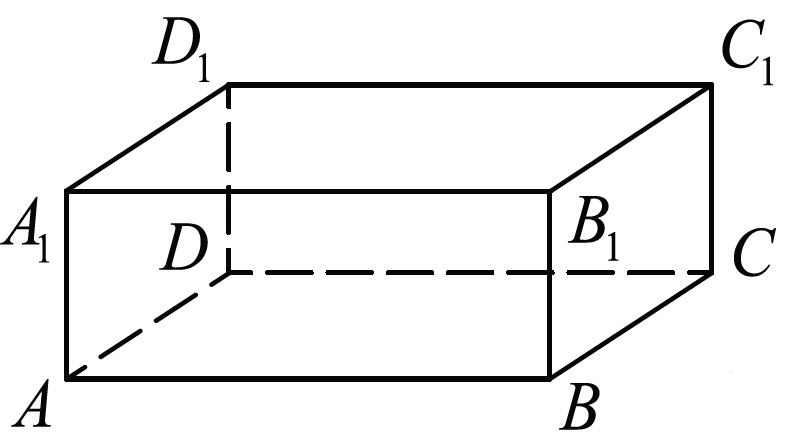
\includegraphics[align=t, width=\linewidth]{\picpath/G101M9L1-1}
		%\end{minipage}
		
	\end{listofex}
\end{class}
%END_FOLD

%BEGIN_FOLD % ====>>_ Домашняя работа 3 _<<====
\begin{homework}[number=3]
	\begin{listofex}
		\item Каждому из четырёх неравенств в левом столбце соответствует одно из решений в правом столбце. Установите соответствие между неравенствами и их решениями. \\
		\begin{minipage}[t]{0.45\linewidth}
			\begin{tasks}
				\task \( x^2+8x+15 \ge 0 \)
				\task \( x^2 - 8x + 15 \ge 0 \)
				\task \( x^2 - 14x - 15 \le 0 \)
				\task \( x^2 + 14x - 15 \le 0 \)
			\end{tasks}
		\end{minipage}
		\hspace{0.02\linewidth}
		\begin{minipage}[t]{0.45\linewidth}
			\begin{tasks}
				\task \( (- \infty; 3 ] \cup [5; + \infty ) \)
				\task \([-1; 15]  \)
				\task \(  (- \infty; -5 ] \cup [-3; + \infty ) \)
				\task \( [-15; 1] \)
			\end{tasks}
		\end{minipage}
		%111M9L1
		\item Имеется два сплава. Первый сплав содержит \(5\%\) меди, второй --- \(12\%\) меди. Масса второго сплава больше массы первого на \(9\) кг. Из этих двух сплавов получили третий сплав, содержащий \(10\%\) меди. Найдите массу третьего сплава. Ответ дайте в килограммах.
		\item Смешав \(11\)-процентный и \(72\)-процентный растворы кислоты и добавив \(10\) кг чистой воды, получили \(31\)-процентный раствор кислоты. Если бы вместо \(10\) кг воды добавили \(10\) кг \(50\)-процентного раствора той же кислоты, то получили бы \(51\)-процентный раствор кислоты. Сколько килограммов \(11\)-процентного раствора использовали для получения смеси?
		\item Имеется два сплава. Первый содержит \(15\%\) никеля, второй --- \(35\%\) никеля. Из этих двух сплавов получили третий сплав массой \(140\) кг, содержащий \(30\%\) никеля. На сколько килограммов масса первого сплава была меньше массы второго?
		\item Имеются два сосуда. Первый содержит \(30\) кг, а второй --- \(15\) кг раствора кислоты различной концентрации. Если эти растворы смешать, то получится раствор, содержащий \(34\%\) кислоты. Если же смешать равные массы этих растворов, то получится раствор, содержащий \(46\%\) кислоты. Сколько килограммов кислоты содержится в первом сосуде?
	\end{listofex}
\end{homework}
%END_FOLD

%BEGIN_FOLD % ====>>_____ Занятие 7 _____<<====
\begin{class}[number=7]
	\title{Подготовка к проверочной}
	\begin{listofex}
		\item Каждому из четырёх неравенств в левом столбце соответствует одно из решений в правом столбце. Установите соответствие между неравенствами и их решениями. \\
		\begin{minipage}[t]{\bodywidth}
			\begin{tasks}
				\task \( \log_2 x \ge 1 \)
				\task \( \log_2 x \le -1 \)
				\task \( \log_2 x \ge -1 \)
				\task \( \log_2 x \le 1 \)
			\end{tasks}
		\end{minipage}
		\hspace{0.02\linewidth}
		\begin{minipage}[t]{\picwidth}
			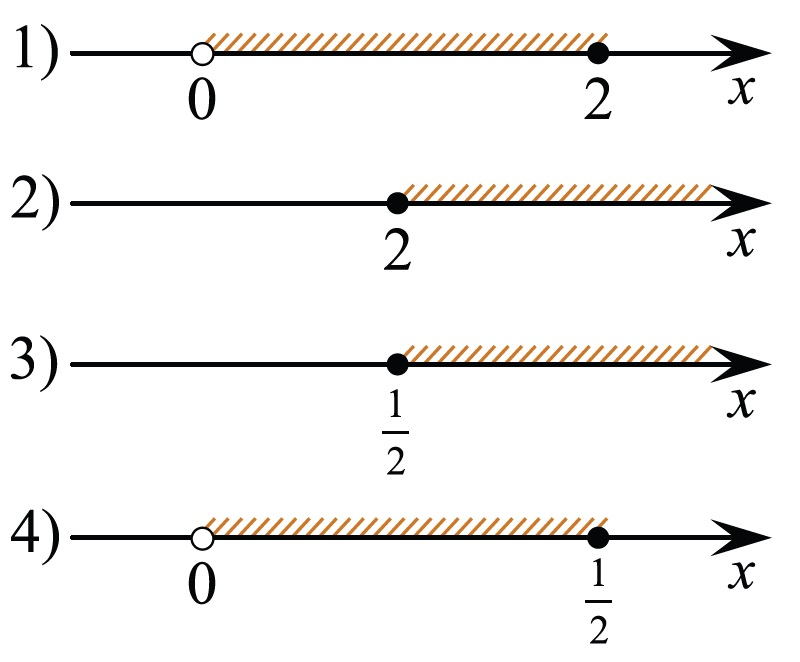
\includegraphics[align=t, width=\linewidth]{\picpath/G101M9L6-3}
		\end{minipage}
	\end{listofex}
\end{class}
%END_FOLD

%BEGIN_FOLD % ====>>_ Проверочная работа _<<====
\begin{exam}
	\begin{listofex}
		\item Проверочная
	\end{listofex}
\end{exam}
%END_FOLD

%BEGIN_FOLD % ====>>_ ДЗ 4 _<<====
\begin{homework}[number=4]
	\begin{listofex}
		\item Смешав \(11\)-процентный и \(72\)-процентный растворы кислоты и добавив \(10\) кг чистой воды, получили \(31\)-процентный раствор кислоты. Если бы вместо \(10\) кг воды добавили \(10\) кг \(50\)-процентного раствора той же кислоты, то получили бы \(51\)-процентный раствор кислоты. Сколько килограммов \(11\)-процентного раствора использовали для получения смеси?
		\item Имеется два сплава. Первый содержит \(10\%\) никеля, второй --- \(35\%\) никеля. Из этих двух сплавов получили третий сплав массой \(150\) кг, содержащий \(30\%\) никеля. На сколько килограммов масса первого сплава была меньше массы второго?
		\item Имеются два сосуда. Первый содержит \(100\) кг, а второй --- \(20\) кг раствора кислоты различной концентрации. Если эти растворы смешать, то получится раствор, содержащий \(67\%\) кислоты. Если же смешать равные массы этих растворов, то получится раствор, содержащий \(77\%\) кислоты. Сколько килограммов кислоты содержится в первом сосуде?
		\item Каждому из четырёх неравенств в левом столбце соответствует одно из решений в правом столбце. Установите соответствие между неравенствами и их решениями. \\
		\begin{minipage}[t]{\bodywidth}
			\begin{tasks}
				\task \( \log_2 x \ge 1 \)
				\task \( \log_2 x \le -1 \)
				\task \( \log_2 x \ge -1 \)
				\task \( \log_2 x \le 1 \)
			\end{tasks}
		\end{minipage}
		\hspace{0.02\linewidth}
		\begin{minipage}[t]{\picwidth}
			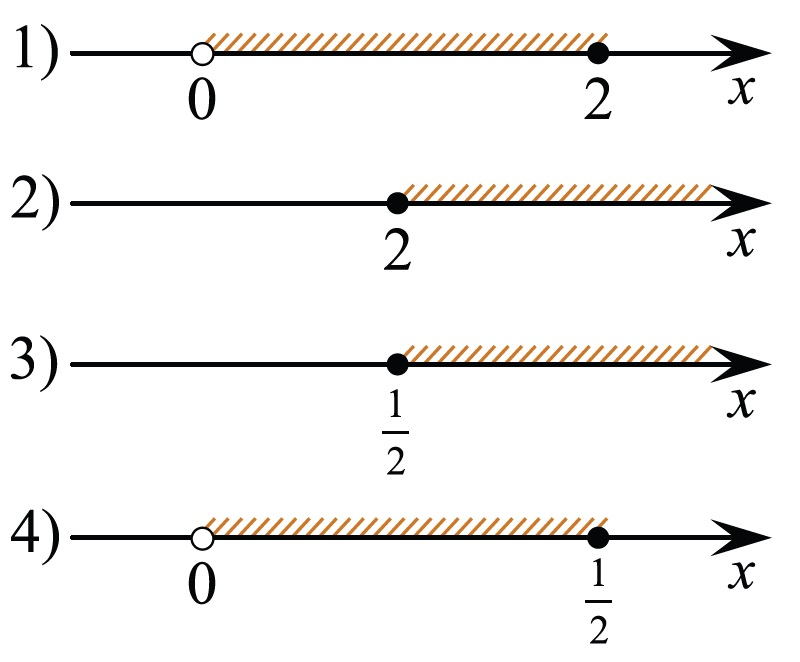
\includegraphics[align=t, width=\linewidth]{\picpath/G101M9L6-3}
		\end{minipage}
		
		\item Каждому из четырёх неравенств в левом столбце соответствует одно из решений в правом столбце. Установите соответствие между неравенствами и их решениями. \\
		\begin{minipage}[t]{0.5\linewidth}
			\begin{tasks}
				\task \( 2^x \ge 2\)
				\task \( 0,5^x \ge 2 \)
				\task \( 0,5^x \le 2 \)
				\task \( 2^x \le 2 \)
			\end{tasks}
		\end{minipage}
		\hspace{0.02\linewidth}
		\begin{minipage}[t]{0.4\linewidth}
			\begin{tasks}
				\task \( x \ge 1 \)
				\task \( x \le 1 \)
				\task \( x \le -1 \)
				\task \( x \ge -1 \)
			\end{tasks}
		\end{minipage}
		\item На прямой отмечены точки \(K, L, M\) и \(N\). \\
		\begin{minipage}[t]{0.8\linewidth}
			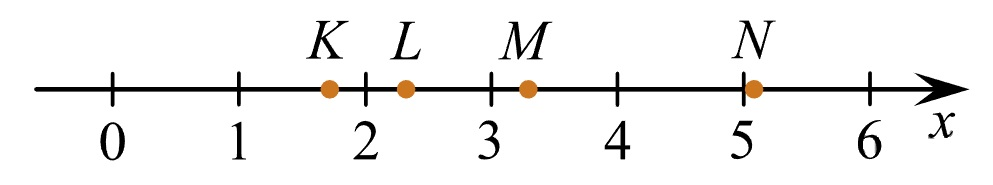
\includegraphics[align=t, width=\linewidth]{\picpath/G101M9H4-1}
		\end{minipage}
		\\
		Установите соответствие между указанными точками и числами из правого столбца, которые им соответствуют.
		\\
		\begin{minipage}[t]{0.4\linewidth}
			\begin{tasks}
				\task \( K \)
				\task \(  L\)
				\task \( M \)
				\task \(  N\)
			\end{tasks}
		\end{minipage}
		\begin{minipage}[t]{0.4\linewidth}
			\begin{tasks}
				\task \( \log_2 10 \)
				\task \( \dfrac{ 7 }{ 3 } \)
				\task \( \sqrt{26} \)
				\task \( 0,6^{-1} \)
			\end{tasks}
		\end{minipage}
		
		%\item На прямой отмечены точки \(A, B, C\) и \(D\).
		%\begin{minipage}[t]{\picwidth}
		%	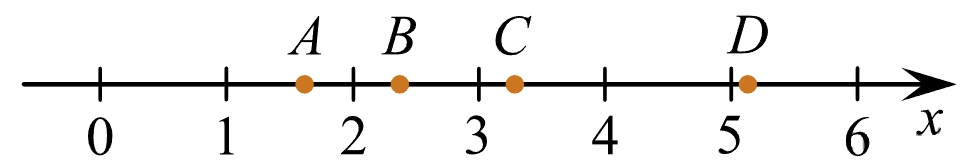
\includegraphics[align=t, width=\linewidth]{\picpath/G101M9H4-2}
		%\end{minipage}
		%\\
		%Установите соответствие между указанными точками и числами из правого столбца, которые им соответствуют.
		%\\
		%\begin{minipage}[t]{0.4\linewidth}
		%	\begin{tasks}
		%		\task \( A \)
		%		\task \(B\)
		%		\task \( C \)
		%		\task \(  D\)
		%	\end{tasks}
		%\end{minipage}
		%\\
		%\begin{minipage}[t]{0.4\linewidth}
		%	\begin{tasks}
		%		\task \( \log_2 10 \)
		%		\task \( \dfrac{ 7 }{ 3 } \)
		%		\task \( \sqrt{26} \)
		%		\task \( 0,6^{-1} \)
		%	\end{tasks}
		%\end{minipage}
		
		
		\item На прямой отмечено число \(m\). \\
		\begin{minipage}[t]{0.8\linewidth}
			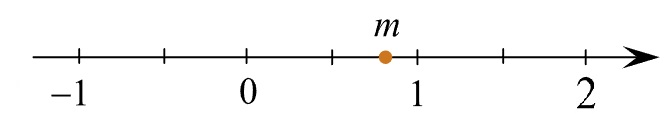
\includegraphics[align=t, width=\linewidth]{\picpath/G101M9H4-3}
		\end{minipage}
		\\
		Каждому из четырёх чисел в левом столбце соответствует отрезок, которому оно принадлежит. Установите соответствие между числами и отрезками из правого столбца.
		\\
		\begin{minipage}[t]{0.4\linewidth}
			\begin{tasks}
				\task \(4-m \)
				\task \(m^2 \)
				\task \( \sqrt{m+1}\)
				\task \( -\dfrac{ 2 }{ m } \)
			\end{tasks}
		\end{minipage}
		\begin{minipage}[t]{0.4\linewidth}
			\begin{tasks}
				\task \( [-3;-2] \)
				\task \( [0;1] \)
				\task \( [1;2] \)
				\task \( [3;4] \)
			\end{tasks}
		\end{minipage}
		
		
		\item Ящик, имеющий форму куба с ребром \(10\) см без одной грани, нужно покрасить со всех сторон снаружи. Найдите площадь поверхности, которую необходимо покрасить. Ответ дайте в квадратных сантиметрах.
		\item Аквариум имеет форму куба со стороной \(40\) см. Сколько литров составляет объём аквариума? В одном литре \(1000\) кубических сантиметров.
		\item Даны две коробки, имеющие форму правильной четырёхугольной призмы, стоящей на основании. Первая коробка в полтора раза ниже второй, а вторая вдвое шире первой. Во сколько раз объём второй коробки больше объёма первой?
		\item Даны две правильные четырёхугольные пирамиды. Объём первой пирамиды равен \(16\). У второй пирамиды высота в \(2\) раза больше, а сторона основания в \(1,5\) раза больше, чем у первой. Найдите объём второй пирамиды.
		\item Пирамида Снофру имеет форму правильной четырёхугольной пирамиды, сторона основания которой равна \(220\) м, а высота --- \(104\) м. Сторона основания точной музейной копии этой пирамиды равна \(44\) см. Найдите высоту музейной копии. Ответ дайте в сантиметрах.
		\item 
		\begin{minipage}[t]{\bodywidth}
			Основанием пирамиды является прямоугольник со сторонами \(4\) и \(5\). Ее объем равен \(80\). Найдите высоту этой пирамиды.
		\end{minipage}
		\hspace{0.02\linewidth}
		\begin{minipage}[t]{\picwidth}
			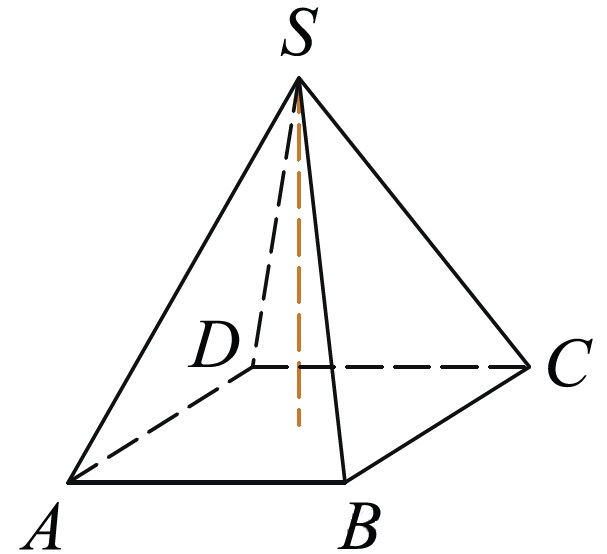
\includegraphics[align=t, width=\linewidth]{\picpath/G101M9L1-3}
		\end{minipage}
		\item В цилиндрический сосуд налили \(6\) куб. см воды. В воду полностью погрузили деталь. При этом уровень жидкости в сосуде увеличился в \(1,5\) раза. Найдите объём детали. Ответ выразите в куб. см.
		\item В треугольнике \(ABC\) \(AC = BC = 25\), \(AB = 40\). Найдите \(\sin A\).
		
		
	\end{listofex}
\end{homework}
%END_FOLD